\documentclass[12pt]{article}
\usepackage[utf8]{inputenc}
\usepackage{color}
\usepackage{polski}
\usepackage{graphicx}
\usepackage{pdfpages}
\usepackage{indentfirst}
\usepackage{geometry}
\usepackage{setspace}
\usepackage[hyphens]{url}
\usepackage[backend=biber]{biblatex}
\usepackage{array}
\usepackage{listings}
\usepackage{float}
\usepackage{listings}
\usepackage{subcaption}

\addbibresource{bibliografia.bib}
\graphicspath{{./zdjecia/}}

\renewcommand\lstlistlistingname{Listingi}

\setstretch{1.5}

\geometry{
 a4paper,
 left=2.5cm,
 top=1.25cm,
 right=2.5cm
}

\definecolor{dkgreen}{rgb}{0,0.6,0}
\definecolor{gray}{rgb}{0.5,0.5,0.5}
\definecolor{mauve}{rgb}{0.58,0,0.82}

\lstset{frame=tb,
  language=Python,
  aboveskip=3mm,
  belowskip=3mm,
  showstringspaces=false,
  columns=flexible,
  basicstyle={\small\ttfamily},
  numbers=none,
  numberstyle=\tiny\color{gray},
  keywordstyle=\color{blue},
  commentstyle=\color{dkgreen},
  stringstyle=\color{mauve},
  breaklines=true,
  breakatwhitespace=true,
  tabsize=3
}

\begin{document}
\begin{sloppypar}

\includepdf{Strona_Tytulowa.pdf}

\tableofcontents
\newpage

\section{Wprowadzenie}
{
  \subsection{Problematyka}
  {
    W dzisiejszych czasach bardzo modnym tematem jest sztuczna inteligencja, która zaczyna się wkradać w każdy aspekt naszego życia.
    Możemy ją spotkać w formie chatów, podpowiedzi do pisanego kodu, asystentów internetowych, systemów rozpoznawania głosów, czy nawet we własnej lodówce!
    Każda firma żeby zaistnieć i pozostać istotną inwestuje w tę część technologii. Jednakże to z czym AI radzi sobie najgorzej są ręce.
    \newline
    W tym projekcie chodzi o stworzenie sieci typu GAN, która pozwoli na generowanie obrazów rąk, w jak najlepszej jakości.
    Dodatkowo sieć ma za zadanie nauczyć się, żeby móc modyfikować istniejące zdjęcia i nadawać im zupełnie inny gest, przy zachowaniu jakości i realizmu.
    Szczególnie ten drugi aspekt pozostaje dla sztucznej inteligencji problematyczny. 
    Myślę, że każdy z nas spotkał się ze zdjęciami, które dosłownie wyglądają, jak żywe, ale to co najczęściej zdradza, że jednak to AI maczało w nim palce są ręce.
    Za długie palce, dziwne ich ułożenie, ilość, czy nawet totalnie odrealniony wygląd. 
    Przeróżne firmy, jak i naukowcy stale ulepszają sieci, i rozwiązania, żeby i to przestało być problemem.
    Niniejsza praca również podejmuje się tego niełatwego zadania.
  }
  \subsection{Cel i zakres pracy}
  {
    Celem niniejszej pracy jest stworzenie sieci neuronowej typu GAN, 
    która pozwoli na generowanie obrazów gestów rąk, w jak najlepszej jakości.
    \newline
    Docelowo również, wygenerowane zdjęcia będą wykorzystywane do stworzenia animacji przechodzenia z jednego gestu w inny.
  }
  \subsection{Struktura pracy}
  {
    Pierwszy rozdział przybliży to czym są sieci neuronowe, a dokładniej typu GAN, jakie są analogiczne rozwiązania, oraz o samym generowaniu zdjęć.
    Następny opowie jakie narzędzia, biblioteki i technologie zostały wykorzystane do realizacji projektu. 
    Trzeci zaś mówi o tym jak wyglądał proces tworzenia projektu. Co po koleji zostało zrobione, jakie po drodze wystąpiły komplikacje, oraz jak zostały rozwiązane i finalnie jak wygląda projekt.
    Przedostatni rozdział to przedstawienie wyników, rezultatów realizowanego projektu, analiza i omówienie ich.
    Ostatni rozdział zawiera wnioski końcowe i podsumowanie.
  }
}

\section{Sieci GAN, analiza konkurencji i techniczne aspekty realizacji}
{
  \subsection{Sieci neuronowe i AI}
  {
    Człowiek od samego początku swojego istnienia jest istotą niesamowicie ciekawą. 
    To ona sprawia, że w głowie ludzi pojawiają się pytania, a co jeśli? 
    A co jeśli to co wiemy to jest tylko część prawdy? Co jeśli jest coś więcej?
    To dzięki zadawaniu sobie przeróżnych pytań przez różne osoby, najczęściej przez największe umysły jakie chodziły po tej ziemii tak dużo udało nam się osiągnąć.
    Poczynająć od wynalezienia koła, silniki parowe, elektryczność, internet aż po loty w kosmos. 
    Niektóre z tych wynalazków łączy kolejny aspekt, to że człowiek chce sobie ułatwiać codzienne zadania. 
    Żeby jak najbardziej zwiększyć swoją produktywność, żeby codziennie czynności nie wchodziły w drogę, albo żeby je po prostu ułatwić czy przyspieszyć. \\
    Kolejnym taki wynalazkiem, który łączy te dwa aspekty jest sztuczna inteligencja. 
    Już od dawien dawna, przeróżne filmy czy książki science-fiction rozbudzały naszą wyobraźnię, o istnieniu robotów, sztucznej inteligencji równej ludzkiej, czy nawet przewyższająca ją. \\
    Do stworzenia pierwszych wzorów, inspiracją była ludzka sieć neuronowa, to jak działa nasz mózg. 
    Takie coś starano się przekuć w pierwszej wzory, pierwsze sieci. Początkowo był to prosty matematyczny opis komórki neuronowej przez McCullocha i Pittsa w 1943 \cite{sztuczna-inteligencja}.
    W połączeniu z zagadnieniem przetwarzania danych mógł modelować proste funkcje logiczne. 
    Dopiero w 1949 roku Hebb sformułował regułę, którą uznaje sie za pierwszą regułę uczenia sztucznych sieci neuronowych\cite{sztuczna-inteligencja}.\\
    Obecnie sieci i modeli sieci jest tysiące. Do najpopularniejszych należą np CNN - Convolutional Neural Network, czy RNN - Recurrent Neural Network.
    W tym projekcie wykorzystujemy sieci typu GAN, czyli Generative Adversarial Network, o której więcej w kolejnym podrozdziale.
  }
  \subsection{Budowa sieci neuronowej}
  {
    Najmniejszą składową sieci neuronowej są oczywiście neurony, te neurony są poukładane po kilka w tak zwane warstwy. 
    Najmniejsza ilość warstw to 3. 
    Składają się z warstwy wejściowej, reprezentuje dane wejściowe w postaci numerycznej, warstwy ukryte, liczba mnoga tu jest celowa, ponieważ ich może wystąpić nieskończenie wiele, to one wykonują obliczenia.
    Ostatnim typem warstwy jest warstawa wyjściowa, ona generuje dane wyjściowe. \\
    Tylko no właśnie dane. Jako, że sieci neuronowe to matematyka, to muszą działać na liczbach także nasze dane muszą być zmienione na liczby, a następnie znormalizowane do zakresu między 0 a 1.
    \begin{figure}[H]
      \centering
      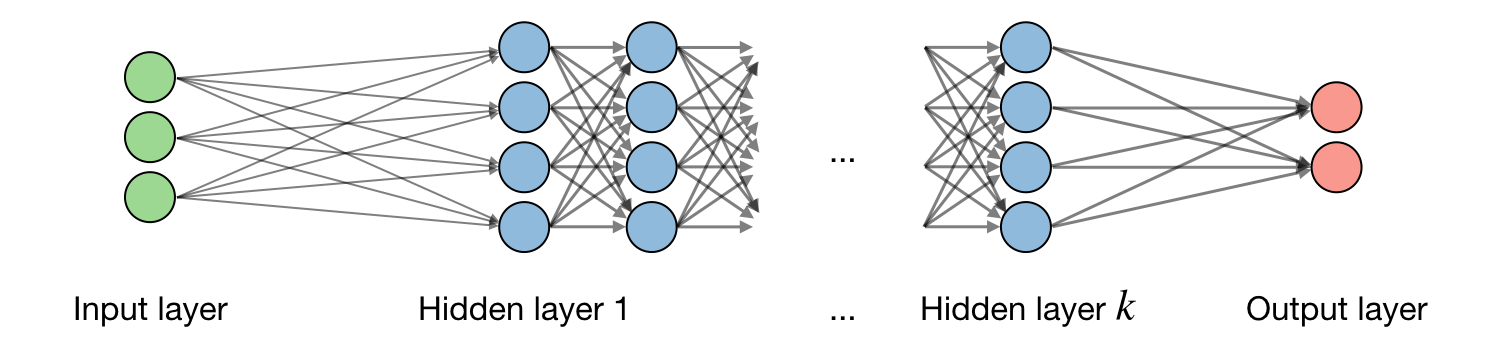
\includegraphics[width=0.9\textwidth]{neural-network-stanford.png}
      \caption{Budowa sieci neuronowej \cite{nlp}}
      \label{fig:nn}
    \end{figure}
    Zajmijmy się teraz najmniejszą częścią sieci, czyli neuronem.
    \begin{figure}[H]
      \centering
      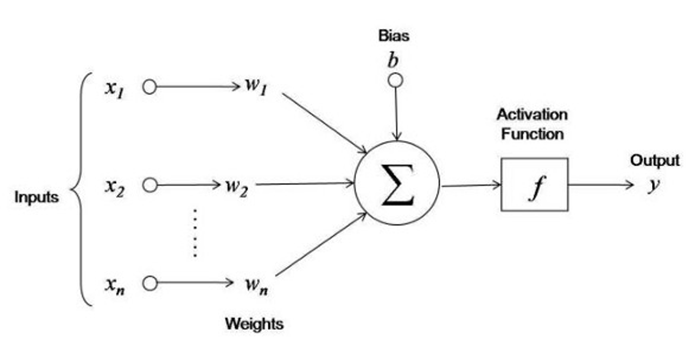
\includegraphics[width=0.9\textwidth]{perceptron.png}
      \caption{Budowa neuronu \cite{nlp}}
      \label{fig:neuron}
    \end{figure}
    "W neuronie wartości sygnałów wejściowych (oznaczone na rysunku jako x1, x2, … , xn) mnożone są przez wagi (oznaczone jako w1, w2,…, wn), a iloczyny są ze sobą dodawane (do wyniku dodawana jest wartość b, która nie jest mnożona przez wartość sygnału wejściowego). 
    Wynik rachunków poddawany jest funkcji aktywacji, która decyduje o ostatecznej wartości wysyłanego sygnału. 
    W najprostszym przypadku może to być funkcja progowa (1 dla wartości dodatnich, 0 dla wartości niedodatnich), która przypomina działanie ludzkiego neuronu: „wysyłam sygnał lub nie”."\cite{nlp}
  }
  \subsection{Sieci typu GAN}
  {
    Sieci GAN czyli Generative Adversarial Network, a tłumacząc na polski, generatywne sieci współzawodnicze.
    Jak sama nazwa wskazuje są to sieci generatywne, czyli generują dane, najczęściej są to obrazy, ale nie ma ograniczeń, mogą być to również np filmiki.
    Sieci GAN składają się tak naprawdę z dwóch sieci, które ze sobą równocześnie współzawodniczą.
    Bardzo często są porównywane do fałszowania pieniędzy, mamy jedną sieć, która się uczy generować jak najdokładniejsze fałszywki, a drugą, która ma za zadanie odrzucać fałszywki.
    Podzielone są na:
    \begin{itemize}
      \item Generator uczy się generować wiarygodne dane i docelowo oszukać diskriminator, że to co generuje jest prawdziwe
      \item Diskriminator, uczy się odróżniać prawdę od fikcji
    \end{itemize}
    \begin{figure}[H]
      \centering
      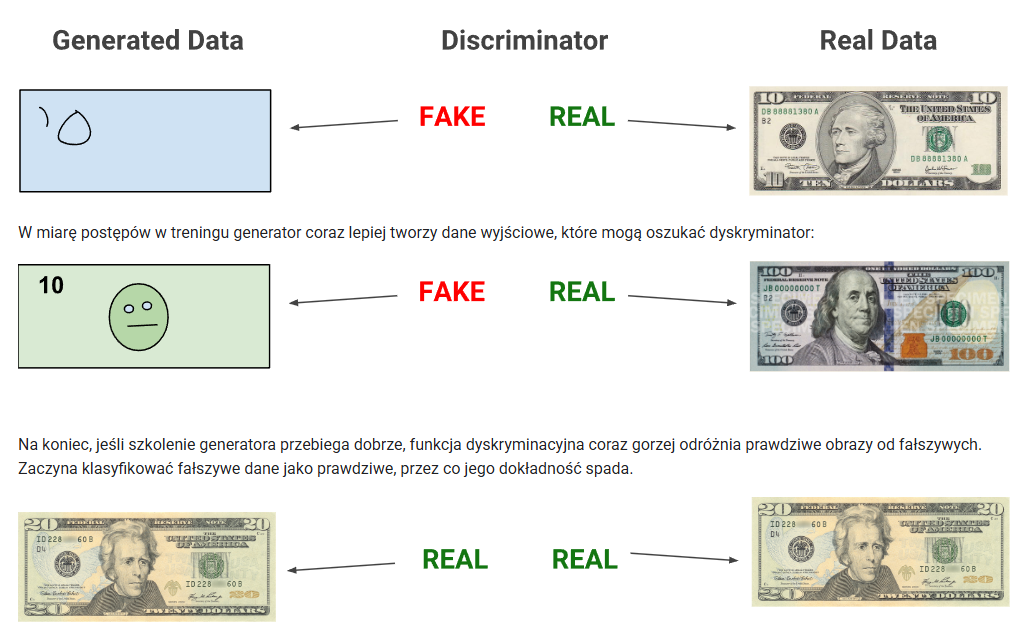
\includegraphics[width=0.9\textwidth]{gan.png}
      \caption{Generative Adversarial Network \cite{google-gan}}
      \label{fig:gan}
    \end{figure}
    \begin{figure}[H]
      \centering
      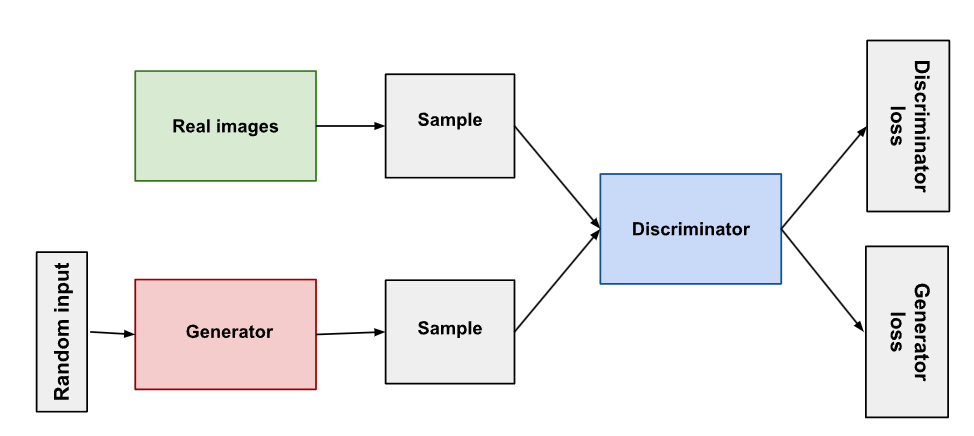
\includegraphics[width=0.9\textwidth]{gan-budowa.png}
      \caption{Ogólny model sieci GAN \cite{google-gan}}
      \label{fig:gan-budowa}
    \end{figure}
    Sieci GAN mają oczywiście swoje pod typy, czy też może framworki, czy jeszcze inaczej już wcześniej stworzone typy tej sieci, które są powszechnie znane i używane.
    Wyróżnić można:
    \begin{itemize}
      \item Pix2Pix jest to sieć, która przetwarza jedno zdjęcie w drugie, co jest istotne w tej sieci to to, że dane musza być sparowane, czyli jeden z obrazów jest obrazem wejsciowym, a drugim obrazem wyjsciowym
      \item CycleGAN jest bardzo podobny do Pix2Pix tylko zbiór danych nie jest sparowany. Można za jego pomocą robić takie translację jak np. z koni zebry
    \end{itemize}
    Ten pierwszy został wykorzystany do stworzenia tego projektu, choć początkowo to ten drugi był używany, ale o tym w oddzielnym rozdziale.
  }
  \subsection{GestureGAN}
  {
    GestureGAN\cite{gesture-gan} jest to propozycja stworzona przez specjalistów z różnych uczelni, takich jak OXform czy Texas State Univerity.
    W swoim założeniu ma robić to samo co sieć stworzona na potrzeby tego projektu, jednakże to jej budowa jest tym co je rozróżnia.
    Była to bardzo duża inspiracja przy tworzeniu projektu, podobnie jak niniejsza sieć wykorzystywany jest mediapipe do ekstrakcji szkieletu. 
    Co je np rozróżnia to, że GestureGAN otrzymuje dwa zdjęcia na wejściu, jedno prawdziwe, drugie samego szkieletu docelowego i ma wyjściu otrzymujemy wygenerowane zdjęcie i pierwotny szkielet.
    Takie rozwiązanie było ok w przypadku ichniego zbioru danych, ponieważ był sparowany, to znaczy ta sama osoba wykonywała wszystkie gesty. 
    Niestety w wykorzystanym przeze mnie zbiorze danych nie było takiej możliwości, dane stały się sparowane nieco sztucznie, ale o tym później.
    Bardzo dużą zaletą tego projektu jest to, że jest bardzo uniwersalny, z każdego gestu jesteśmy w stanie uzyskać każdy gest.
    \begin{figure}[H]
      \centering
      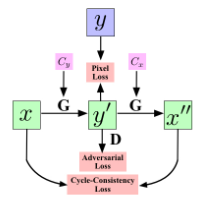
\includegraphics{gesture-gan.png}
      \caption{Model GestureGAN \cite{gesture-gan}}
      \label{fig:gesture-gan-budowa}
    \end{figure}
    i tu jeszcze przykładowe efekty i możliwości GestureGAN\cite{gesture-gan}.
    \begin{figure}[H]
      \centering
      \includegraphics[width=0.9\textwidth]{gesturegan-framework.jpg}
      \caption{Zdjęcie wygenerowane przez GestureGAN \cite{gesture-gan}}
      \label{fig:gesture-gan-przyklady}
    \end{figure}
    Ten projekt stanowiłby bardzo dobrą baze, generuje wyraźnie i zróżnicowane gesty rąk, jest bardzo uniwersalny, ale problem zaczyna się już na początku.
    Zbiór danych, który tutaj jest wykorzystywany jest niedostępny, albo wymaga dodatkowych dostępów. Nie wszystkie dane też są dostępne, choćby zdjęcia szkieletów.
    Te dane, które były dostępne, było ich po prostu za mało, plus możliwości tego projektu nie są aż tak potrzebne do realizacji tego, plus nie wiadomo jak z rozszerzalnością kodu.
    Dlatego najlepszym rozwiązaniem było przygotowanie własnego zbioru danych, własnego modelu i metodą prób i błędów, dochodzenie do rozwiązania.
  }
  \subsection{PoseGAN}
  {
    PoseGAN\cite{pose-gan} jest dość zbliżony do GestureGAN, jednakże ma zasadniczą różnicę w swoim zastosowaniu.
    Tak jak GestureGAN, jak sama nazwa wskazuje służy do generowania gestów rąk, tak PoseGAN służy do generowania całych poz ludzkich.
    Także zakres jest większy jednakże przez fakt, że nie ma skupienia na dłoniach dokładność wykonywanego gestu nie ma tu znaczenia.
    Jednakże jest to zdecydowanie najbliższe wykonywanemu projektowi.
    \begin{figure}[H]
      \centering
      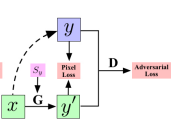
\includegraphics{pose-gan.png}
      \caption{Model PoseGAN \cite{pose-gan}}
      \label{fig:pose-gan-budowa}
    \end{figure}
    \begin{figure}[H]
      \centering
      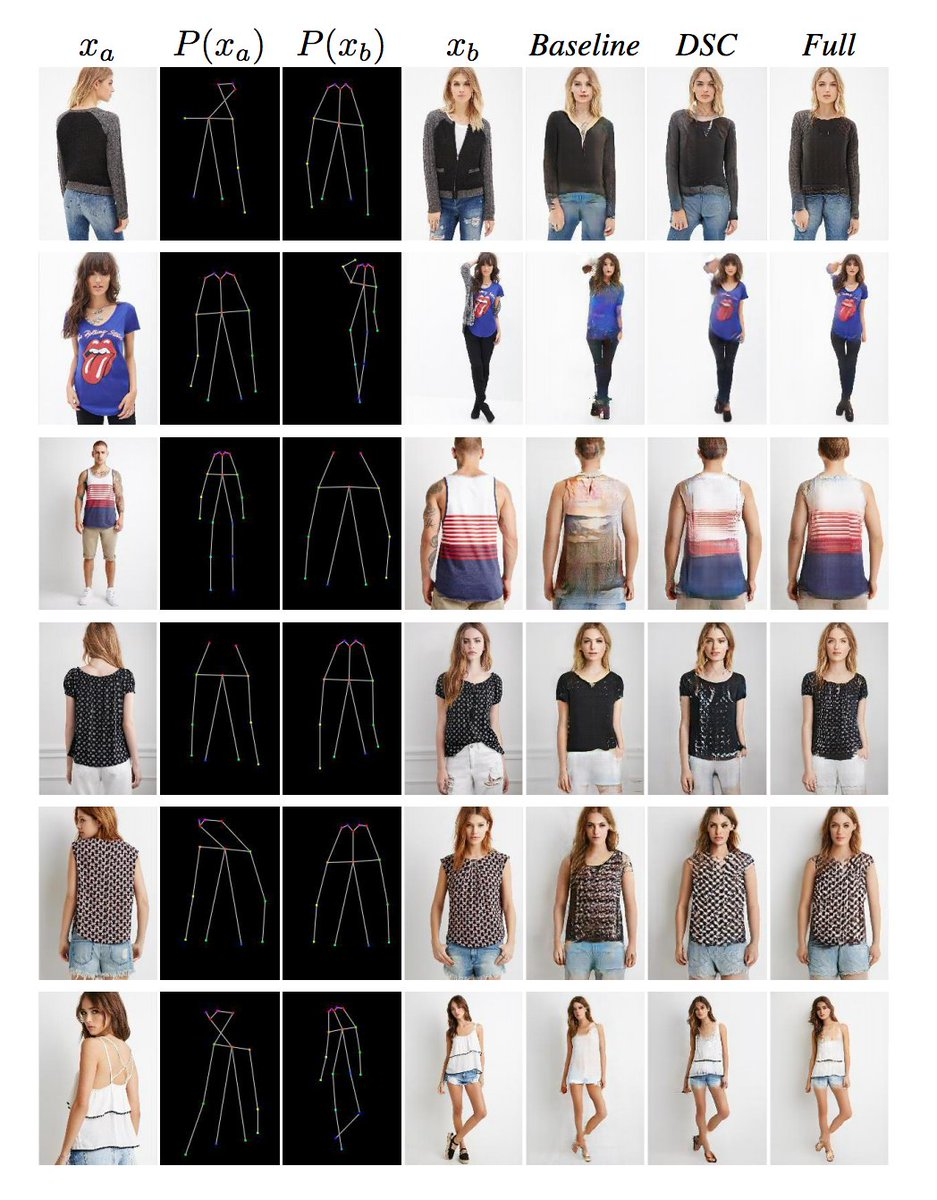
\includegraphics[width=0.9\textwidth]{pose-gan-ex.jpg}
      \caption{Zdjęcie wygenerowane przez PoseGAN \cite{pose-gan}}
      \label{fig:pose-gan-przyklady}
    \end{figure}
    Projekt jest niewątpliwie bardzo imponujący jednakże no właśnie skupia się na czymś kompletnie innym. 
    Tak jak widać na \ref{fig:pose-gan-przyklady} dłonie nawet nie są wyszczególnione na szkielecie, a przerabianie, a w zasadzie dorabianie takiego elementu byłoby zbyt czasochłonne.
    Sieć i tak by musiała się uczyć wszystkiego od nowa, plus no właśnie do końca interesuje nas cały ludzki szkielet. Dlatego niezbędne było stworzenie własnego projektu.
  }
}

\section{Narzędzia i technologie wybrane do realizacji projektu}
{
  \subsection{Python}
  {
    Językiem programowania wykorzystanym do realizacji projektu jest Python. 
    Jest to bardzo oczywisty wybór, ponieważ jest to najpopularniejszy język programowania do tworzenia sieci neuronowych w dzisiejszych czasach.
    Przybliżmy go jednak, według oficjalnej dokumentacji, jest "łatwym do nauczenia się i potężnym językiem programowania. 
    Posiada wydajne struktury danych wysokiego poziomu oraz proste, ale skuteczne podejście do programowania obiektowego"\cite{python-docs}.
    Co niejako wyróżnia go na tle innych języków to fakt, że jest dynamicznie typowany oraz jest językiem interpetowanym. 
    To oznacza, że nie posiada kompilatora a interpeter, który nie kompiluje programu do pliku wykonywalnego, a kod jest wykonywany w czasie rzeczywistym.
    Czyni to Python językiem łatwym w testowaniu, kompilowaniu czy wykonywaniu, przenośny, co oznacza, że ten sam kod uruchomi się niezależnie od systemu operacyjnego czy urządzenia.
    Sam język Python jest zbudowany na bibliotece C, co oznacza, że jest bardzo szybki i wydajny. 
    Został stworzony przez Guido van Rossuma w roku 1991.
    Co ciekawe jego nazwa wywodzi się z starych serii skeczów grupy Monty Python’s Flying Circus, 
    a zyskał na popularności w momencie gdy firma Google, powiedziała, że wykorzystuje go do własnych, wewnętrzych celów.
    \newline
    Jednakże czemu akurat to on jest najczęściej wykorzystany do AI? Odpowiedź jest tak prosta jak sam Python jest prosty.
    Wynika to z tego, że Python ma bardzo prostą i czytelną składnię, co pozwala developerom skupianie się na logice i samym problemie, a nie na składni\cite{python-ai}.
    Dodatkowo Python sam w sobie nie wymaga dużej ilości kodu. Najprostsza sieć neuronowa może zostać stworzona i uruchomiona w zaledwie 4 linijki!
    Kolejnym powodem przemawiającym dlaczego to własnie Python jest najczęściej używany, 
    jest bardzo duża ilość bibliotek, czy to wbudowanych, czy stworzonych przez społeczność. 
    Biblioteki takie jak NumPy, SciPy, Matplotlib, czy wykorzystane w tym projekcie PyTorch czy MediaPipe, o których będzie w kolejnych podroździałach.
    Także kolejnym i osatnim już aspektem, o którym chcę wspomnieć, jest wyżej wymieniona społeczność. 
    To dzięki dużej liczbie osób i ogromnym zebranym doświadczeniu, tworzenie dowolnego projektu staje się znacznie prostsze. 
    Praktycznie każdy projekt, aspekt projektu czy problem natrafiało wcześniej duża część ludzi, dzięki czemu możemy szybko i sprawnie rozwiązaywać problem.
  }
  \subsection{PyTorch}
  {
    "PyTorch to w pełni funkcjonalny framewordk do tworzenia modeli do deep learningu, kóry jest typem machine learningu, najczęściej wykorzystywanym w aplikacjach takich jak
    rozpoznawanie obrazów czy procesowanie języka."\cite{pytorch-nvidia} 
    Biblioteka ta została napisana w Pythonie, przez developerów z Facebook AI Research, oraz ma doskonałe wsparcie do wykorzystywania GPU, szczególnie dla GPU od firmy Nvidia, który posiadam.
    Co czyni ją idealną biblioteką dla tego projektu. Jednak projekt dotyczy generowania obrazów rąk, czyli dobre wykorzystanie GPU jest bardzo wskazane.
    Początkowo jednak używana była konkurencyjna biblioteka, a dokładnie Tensorflow, jednakże była zdecydowanie wolniejsza i mniej klarowna od PyTorch co zaważyło na finalnym wyborze.
  }
  \subsection{MediaPipe}
  {
    "MediaPipe Solutions to zestaw bibliotek i narzędzi, które umożliwiają szybkie stosowanie w aplikacjach technik sztucznej inteligencji (AI) i uczenia maszynowego (ML). "\cite{mediapipe}
    Opis ten pochodzi z oficjalnej dokumentacji Mediapipe, jednakże sam opis jest zbyt ogólny. 
    Ta biblioteka ma masę możliiwości i zastosować. Do nich można zaliczyć np. rozpoznawanie obrazu, nie chcemy pisać sieci do rozpoznawania, czy na danym obrazku jest pies czy kot? Mediapipe daje gotowe rozwiązanie!
    Poza tym do wyboru jest też klasyfikacja obrazu, segmentacja obrazu, wykrywanie twarzy, rozpoznawanie gestu, oraz to co było niezbędne w tym projekcie to wykrywanie rąk.
    To dzieki tej bibliotece udało się wyłuskać szkielet ręki na każdym z obrazów ze zbioru danych, nałożyć go na zdjęcie wraz z maską i przekazane do modelu. 
    Później te informacje były użyte do tworzenia kolejnych klatek animacji przechodzenia z jednego gestu w drugi.
  }
  \subsection{OpenCV}
  {
    OpenCV jest to biblioteka do machine learningu oraz computer vision, posiada w swoim arsenale dostęp do takich narzędzi jak wykrywanie i rozpoznawanie twarzy,
    identyfikowanie obiektów, śledzenie ruchów kamery, śledzenie obiektów 3D, usuwanie czerwonych oczu ze zdjęć, czy nawet łączenie zdjęć razem, by uzyskać obraz całej sceny o wysokiej rozdzielczości.\cite{opencv}
    Jednak to żadna z tych funkcji nie została użyta w projekcie. 
    Wykrywanie i tworzenie szkieletu to zadanie Mediapipe, tworzenie modelu to działka PyTorch. 
    OpenCV miał znacznie prostsze zadanie, został wykorzystany do ładowania zdjęć, czy to dla preprocessingu, czy już bezpośrednio do modelu.
    Dalej zapisywał każdy kolejny obraz w zależności od epoki, dzięki czemu można było śledzić poczynania i na koniec sklejał wszystkie klatki i tworzył z nich animację.
  }
}

\section{Proces tworzenia projektu}
{
  \subsection{Dobór zbioru danych}
  {
    Pierwszym i bardzo, ale to bardzo ważnym krokiem jest wybór zbioru danych. 
    Zbiór danych to podstawa projektu, nasz model jest tyle wart ile nasz dataset i jego obróka. 
    To od niego będzie zależeć zarówno to jak długo sieć będzie się uczyć, ale przede wszystkim jakie osiągnie rezultaty. 
    Gdy nasz zbiór jest wyraźny, najlepiej dane są sparowane, to nasza sieć bardzo szybko zrozumie na czym polega różnica i na czym powinna się skupiać. \\
    Poszukiwania były zaskakująco problematyczne, głównie ze względu na słabą współpracę z biblioteką Mediapipe. 
    Często te zdjęcia to były białe plamy na czarnym tle, przez co ciężko było nawet rozróżnić ustawienie dłoni czy choćby palce.
    Inny dataset prezentował zdjęcie robione kamerą nocną, co w zasadzie prowadziło do takich samych rezultatów jak w poprzednio wspomnianym zbiorze.
    Mediapipe nie umiał wychwycić gdzie znajduje się dłoń, palce czy stawy. 
    Kolejne próby były już na zbiorze przedstawiającym zdjęcia liter przedstawianych w języku migowym. 
    Ten zbiór był dobry, ze wględu na to, że przedstawiał same dłonie, na jednolitym tle, był sparowany. 
    Jednakże co skreśliło go, to fakt, że tych zdjęć było po prostu za mało. 
    Dla problemu takiego jak generowanie gestów, tych zdjęć musi być dużo. Tam było ich mniej więcej 30 na gest. Jest to dużo za mało \\
    Finalnie wybór padł na zbiór HaGrid \cite{nuzhdin2024hagridv21mimagesstatic}. \\
    Ten zbiór nie jest niestety sparowany, jednakże posiada na tyle dużo zalet, że warto było go wybrać. \\
    Po pierwsze jest ogromny, cały posiada aż 1.5TB, 1 086 158 zdjęć w FullHD, podzielonych na 33 klasy gestów. 
    Co więcej do zbioru jest dołączony plik json dla każdego gestu, poniżej przykładowy fragment dla jednego zdjęcia:
    \begin{lstlisting}
      "04c49801-1101-4b4e-82d0-d4607cd01df0": {
        "bboxes": [
            [0.0694444444, 0.3104166667, 0.2666666667, 0.2640625],
            [0.5993055556, 0.2875, 0.2569444444, 0.2760416667]
        ],
        "labels": [
            "thumb_index2",
            "thumb_index2"
        ],
        "united_bbox": [
            [0.0694444444, 0.2875, 0.7868055556, 0.2869791667]
        ],
        "united_label": [
            "thumb_index2"
        ],
        "user_id": "2fe6a9156ff8ca27fbce8ada318c592b",
        "hand_landmarks": [
                [
                    [0.37233507701702123, 0.5935673528948108],
                    [0.3997604810145188, 0.5925499847441514],
                    ...
                ],
                [
                    [0.37388438145820907, 0.47547576284667353],
                    [0.39460467775730607, 0.4698847093520443],
                    ...
                ]
            ]
        "meta": {
            "age": [24.41],
            "gender": ["female"],
            "race": ["White"]
        }
    \end{lstlisting}
    Jak widzimy znajduje się tu bardzo dużo przydatnych informacji. Do najważniejszych należą:
    \begin{itemize}
      \item bboxes - są ta koordynaty na jakim obszarze znajdują się dłonie, przydało się to do przycinania zdjęć do wielkości 256x256, która jest standardem dla sieci GAN
      \item labels - dzięki temu wiadomo było którą dłoń wykorzystać do analizy czy też przetwarzania obrazu
      \item hand landmarks - to koordynaty położenia palca, stawów, oraz dłoni
    \end{itemize}
    Tak jak można zauważyć jest to doskonały zbiór danych, do ideału brakuje jednego, żeby był sparowany, ale i to nie jest problem, o czym więcej w rozdziale o preprocessingu. 
  }
  \subsection{Wybór architektury sieci}
  {
    Wybór architektury był nieco uproszczony, bo z założenia projekt wymaga użycia sieci GAN, jednakże podtypów sieci jest dużo.
    Początkowo wybrany został CycleGAN, w zwiazku z tym, że wybrany zbiór nie był sparowany, a CycleGAN dzięki dodatkowej funkcji straty, wykorzystuje 
    utratę spójności cyklu żeby trening nie musiał się odbywać na sparowanych danych. 
    Jako bazę posłużył tutorial z oficjalnej dokumentacji Tensorflow \cite{cyclegan-tf} (wtedy jeszcze to właśnie ta biblioteka była wybrana).
    Z założenia wszystko wydawało się że powinno zadziałać. Na tutorialu robione są z koni zebry, czy z jabłek pomarańcze. 
    To w zasadzie czemu miałoby sobie nie poradzić z gestami?\\
    Rzeczywistość okazała się być bardzo brutalna.
    \begin{figure}[H]
      \centering
      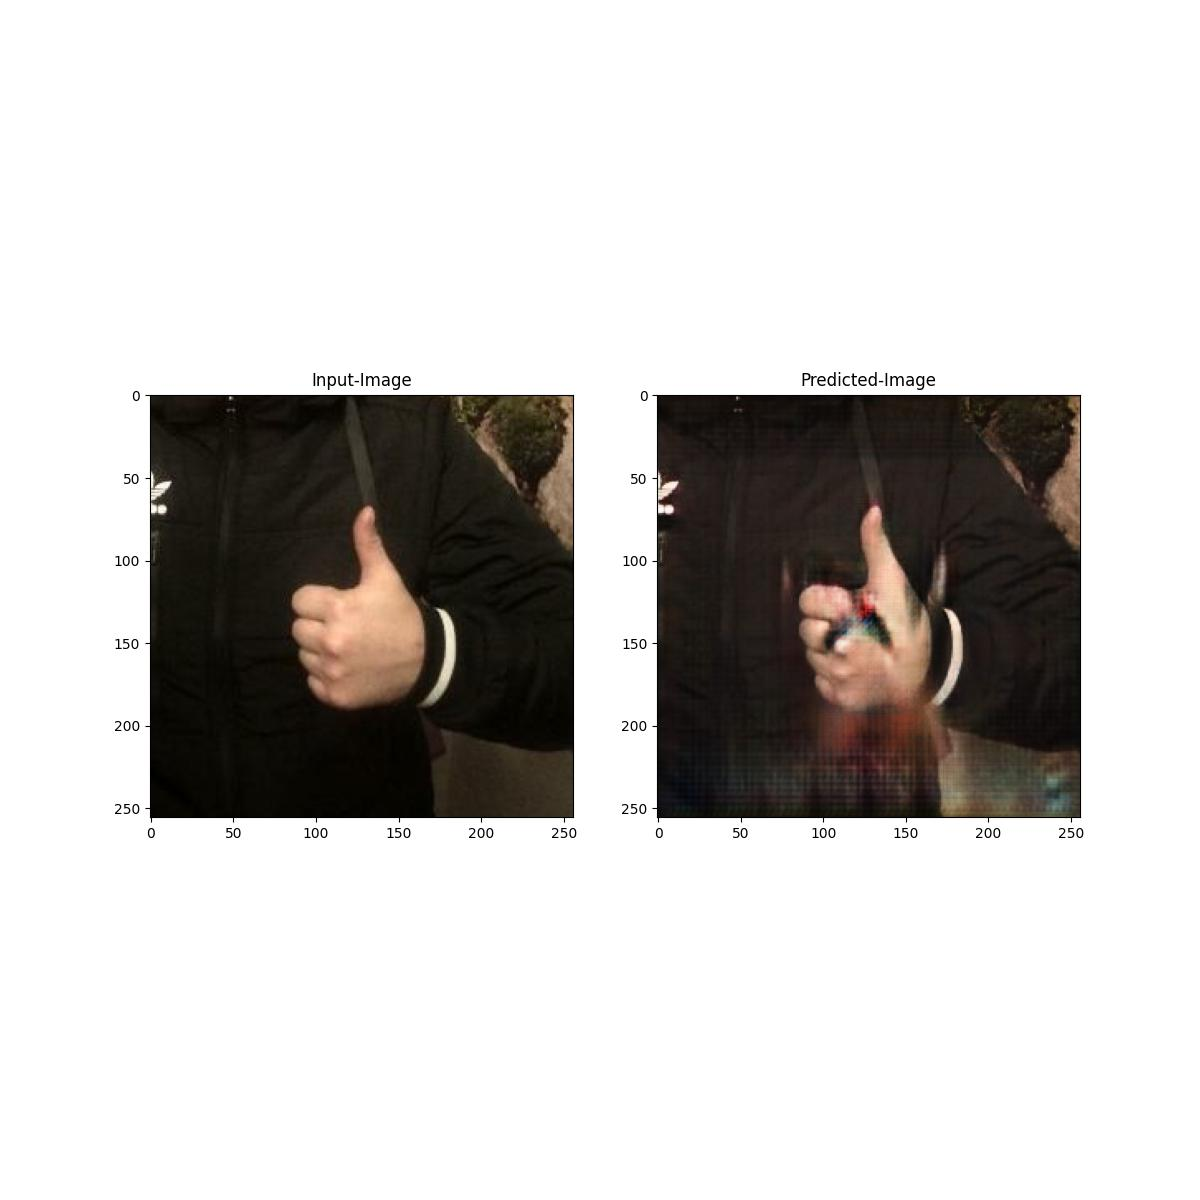
\includegraphics[width=0.9\textwidth]{cycle-gan-45.jpg}
      \caption{Zdjęcie wygenerowane przez CycleGAN, po 45 epokach \cite{cyclegan-tf}}
      \label{fig:cycle-gan-przyklad}
    \end{figure}
    Na pozór wydawać by się mogło, że to zdjęcie jest ok, sieć kombinuje i dosyć wiernie odtworzyła ręke, jedynie pojawiają się artefakty.
    No tak, ale nie takie było jej zadanie. 
    Ona powinna nałożyć nowy gest, ponownie wydawać by się mogło, że zaczyna dobrze kombinować, bo artefakty pojawiają się na dłoni. 
    Tylko niestey przy przeróżnych konfiguracjach parametrów, ilości puszczanych epok, czy zmian, nie udało się zmusić sieć do manipulacji gestami.
    Z tego powodu trzeba było coś zmienić, najwyraźniej zbiór jest zbyt zróżnicowany, tła są inne, przedstwiają innych ludzi itd, żeby CycleGAN sobie poradził. \\
    Więc wybrane zostało inne podejście. Nastąpiła zmiana architektury na Pix2Pix i zmanipulowany został zbiór żeby uczynić go sparowanym. 
    Dokładnie co zostało zrobione jest w kolejnym rozdziale. W dużym skrócie, na ręke z danym gestem, została, na dłoń, nakładana maska i na nią szkielet gestu.
    Co czyni nasz zbiór sparowanym i idealnym kandydatem dla Pix2Pix.
  }
  \subsection{Preprocesowanie danych}
  {
    Preprocesowanie zaczeło się od najprostszej, a zarazem bardzo ważnej części. Przycięcia zdjęć do wielkości 256x256, czyli standardu dla sieci GAN.
    \begin{figure}
      \begin{subfigure}{.5\textwidth}
        \centering
        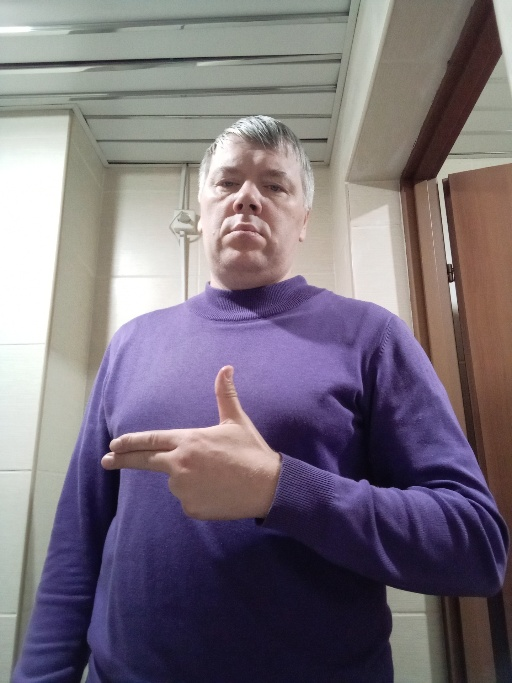
\includegraphics[width=.8\linewidth]{orig.jpg}
        \label{fig:original}
      \end{subfigure}%
      \begin{subfigure}{.5\textwidth}
        \centering
        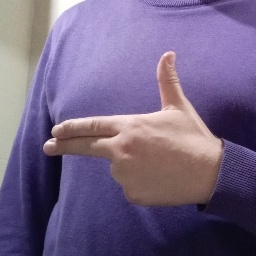
\includegraphics[width=.8\linewidth]{cropped.jpg}
        \label{fig:cropped}
      \end{subfigure}
      \caption{Przykłady przed i po przycięciu}
      \label{fig:orig-crop}
    \end{figure}
    Takie zdjęcia stanowiły początkowy input i zdjęcie docelowe dla sieci. 
    Jednakże jak zostało opisane w podrozdziale o wyborze architektury, to było za mało. \\
    Następnie idąc za przykładem z GestureGAN \cite{gesture-gan}, kolejną próbą było przekazywanie sieci zarówno zdjęcia oryginalnego, jak i oddzielnie zdjęcia docelowego gestu, ale w formie szkieletu na czarnym tle.
    \begin{figure}[H]
      \centering
      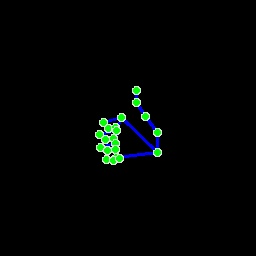
\includegraphics{landmark.jpg}
      \caption{Wygenerowane zdjęcie szkieletu dłoni}
      \label{fig:landmark}
    \end{figure}
    Kolejnymi próbami obróbki zdjęć było usuwanie tła, a w zasadzie rozmazywanie go, przez wycięcie za pomocą biblioteki rembg \cite{rembg}.
    Która to pozwala na wykrycie i usuniecie tła z obrazu. Dłoń i część, która powinna zostać jest wykrywana przy wykorzystaniu MediaPipe. \\
    Tu przykład po takiej obróbce:
    \begin{figure}
      \begin{subfigure}{.5\textwidth}
        \centering
        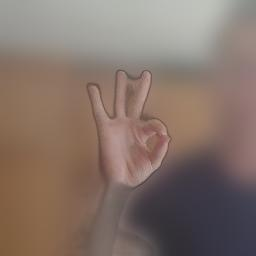
\includegraphics[width=.8\linewidth]{blurred_just_hand.jpg}
        \label{fig:just-hand}
      \end{subfigure}%
      \begin{subfigure}{.5\textwidth}
        \centering
        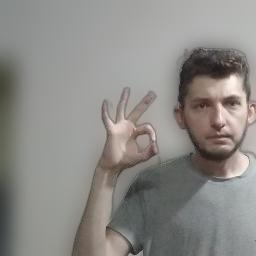
\includegraphics[width=.8\linewidth]{blurred.jpg}
        \label{fig:blurred}
      \end{subfigure}
      \caption{Przykłady po obróbce tła}
      \label{fig:blurred-pre}
    \end{figure}
    Jak widzimy na obrazkach powyżej, efekt jest bardzo różny. Ciężko było o jednoznaczne wykrywanie ręki. 
    Raz zostawała sam ręka, raz wraz z człowiekiem, jeszcze innym razem potrafił zostać sam człowiek. 
    Efekty były mało zadowalające, jednakże, mimo wszystko takie dane również zostały wypróbowane, ponownie nie przynosząc żadnych rezultatów. \\
    Pomimo licznych niepowodzeń i ślepych zaułków, narodził się jeszcze jeden, finalny pomysł. Stworzenie zbioru danych sparowanego, w nieco sztuczny sposób.
    Każde zdjęcie dłoni zostało przepuszczone przez OpenCV i MediaPipe, w celu wykrycia, nałożenia maski a następnie szkieletu gestu. Dając następujący przykład:
    \begin{figure}[H]
      \centering
      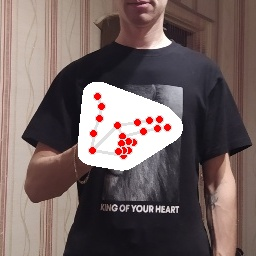
\includegraphics{no_hand.jpg}
      \caption{Przykład zdjęcia z nałożoną maską i szkieletem gestu}
      \label{fig:mask}
    \end{figure}
    Funkcja nakładająca maski jest na tyle uniwersalna, że może przyjąć dowolny kolor i możemy przekazać jej jako parametr, jak duży obszar ma zająć. 
    Jednakże każde zdjęcie jest różne dlatego niezbędne było dobranie jednego rozmiaru maski, która będzie pasować dla znacznej większości obrazów. 
    Tak przygotowane zdjęcia, a w zasadzie zbiór danych posłużył do treningu i testowania sieci.
  }
  \subsection{Modelu i animacja gestu}
  {
    Tesotowanie
  }
}

\section{Wyniki i dyskusja}
{
  wyniki
}

\section{Podsumowanie}
{
  \subsection{Zalety i wady przyjętych rozwiązań}
  {
    Zalety
  }
  \subsection{Napotkane trudności}
  {
    trudności
  }
  \subsection{Możliwości rozwoju}
  {
    rozwoj
  }
  \subsection{Wnioski końcowe}
  {
    wnioski
  }
}

\clearpage
\printbibliography[
  heading=bibintoc,
  title={Bibliografia}
]

\clearpage
\listoffigures

\clearpage
\listoftables

\clearpage
\addcontentsline{toc}{section}{Listingi}
\lstlistoflistings

\end{sloppypar}
\end{document}